\section{Das Innere-Punkte-Verfahren}


\begin{minipage}[h]{0.7\textwidth}
\subsection{Einleitung}
Innere-Punkte-Verfahren sind Algorithmen für die Optimierung von linearen und quadratischen Programmen. Im Vergleich bsp. Zum Simplex-Verfahren zeichnet sich das Innere-Punkte-Verfahren durch schnellere Konvergenz bei dünn besetzten Problemen aus. Im Gegensatz zum Simplex, wo der Algorithmus den Kanten folgt, geht das Innere-Punkte Verfahren den inneren Punkten nach bis zum Optimum (respektive zu dem Ort mit einer genügend kleinen Abweichung).
\end{minipage}
\begin{minipage}[h]{0.3\textwidth} 
  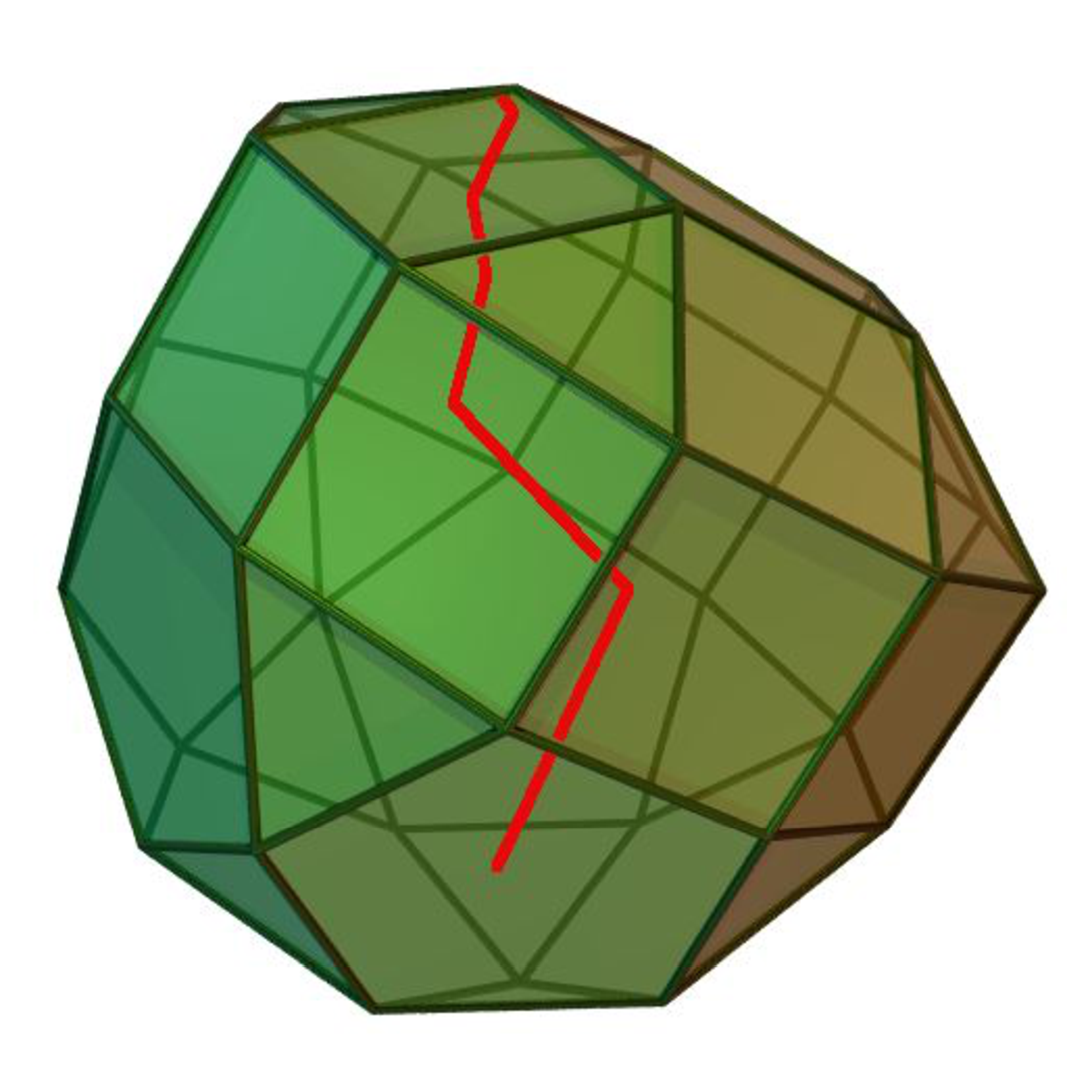
\includegraphics[scale=0.3]{./images/Interior-point-method-three-dimensions.pdf}
\end{minipage}\Uparrow

	
	
\subsection{Idee der Strafterme}

Vielfach gibt es für den zu optimierenden Vektor x eine untere und eine obere Grenze (lb, ub) als Nebenbedingung. Damit diese NB nicht verletzt wird, braucht es ein Strafverfahren und das funktioniert so: Bestrafe die Verletzung der NB in der ZF mit einem Strafterm, der mit einem Strafparameter gewichtet wird, und löse eine Folge mit dieser ZF für wachsenden Strafparameter, bis die Verletzung klein genug ist.\\
\\
\textbf{Strafterm: } $\mu \cdot \log{(x-x_0)}$\\
\\
Der Strafterm soll sich bei der Suche nach einem Minimum extrem vergrössern, sobald sich $x$ dem Grenzwert $x \mapsto x_0$ annähert. Da $-log(x)$ für $x\mapsto 0$ unendlich ergibt sich ein sehr grosser Wert für die ZV, es kann also kein Minimum mehr gefunden werden. Mit dem Strafparameter u kann man die die Genauigkeit erhöhen, je kleiner u, desto weniger fallen die Strafterme bei der ZV ins Gewicht. Die Strafterme werden in der Octave-Funktion automatisch verarbeitet. Es müssen nur die Grenzen als Vektoren angegeben werden (lb= lower bound; ub = upper bound)
\\
\\
Je kleiner $\mu$ gewählt wird, desto kleiner wird der Fehler durch die Strafterme, ausgenommen wenn x an die Grenzen kommt $x \mapsto x_0$, dann geht $f \mapsto \infty$. Für $\mu \mapsto 0$ resultiert die Zielfunktion mit Ausnahme der zwei Extremalstellen bei $x=2$ und $x=4$. Jetzt muss also nur noch dafür gesorgt werden, dass der Punkt X zu Beginn zwischen den Barrieren liegt!	
\\
\\
\textbf{Allgemein:} Min($c^t \cdot x - \mu \cdot \sum_{i=1}^n{log(x_i - x_{io})}$)    und    Max($c^t \cdot x + \mu \cdot \sum_{i=1}^n{log(x_i - x_{io})}$)
\\
\\
\\
\\
\textbf{Beispiel:} Suche das Minimum der Funktion $f=x^2-2x$ mit den Grenzen $x\in]2;4[$\\
\begin{minipage}[t]{6.0cm}
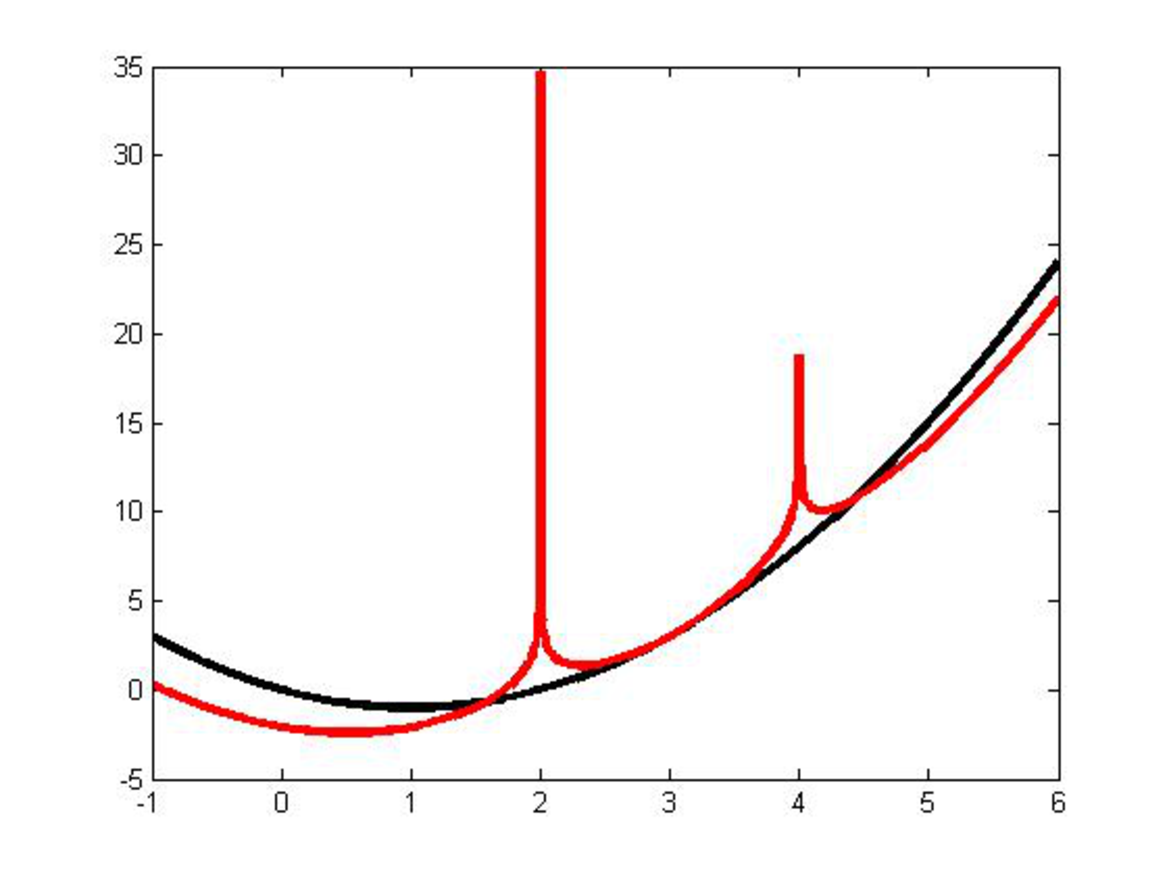
\includegraphics[width=6.0cm]{./images/ln-barrieren-u=1.pdf}\\
	\end{minipage}
	\hspace{0.1cm}
	\begin{minipage}[t]{6.0cm}	
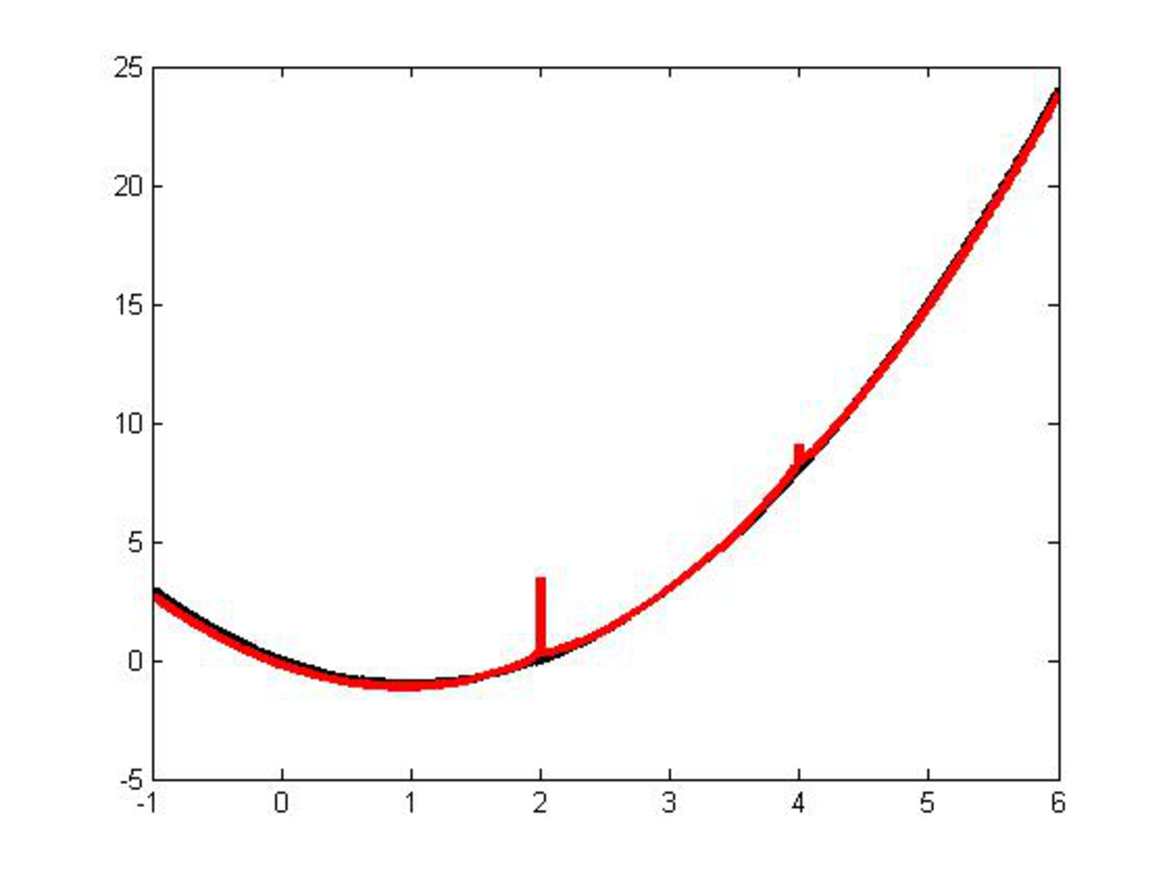
\includegraphics[width=6.0cm]{./images/ln-barrieren-u=0_1-1.pdf}\\
	\end{minipage}
	\hspace{0.1cm}
	\begin{minipage}[t]{6.0cm}	
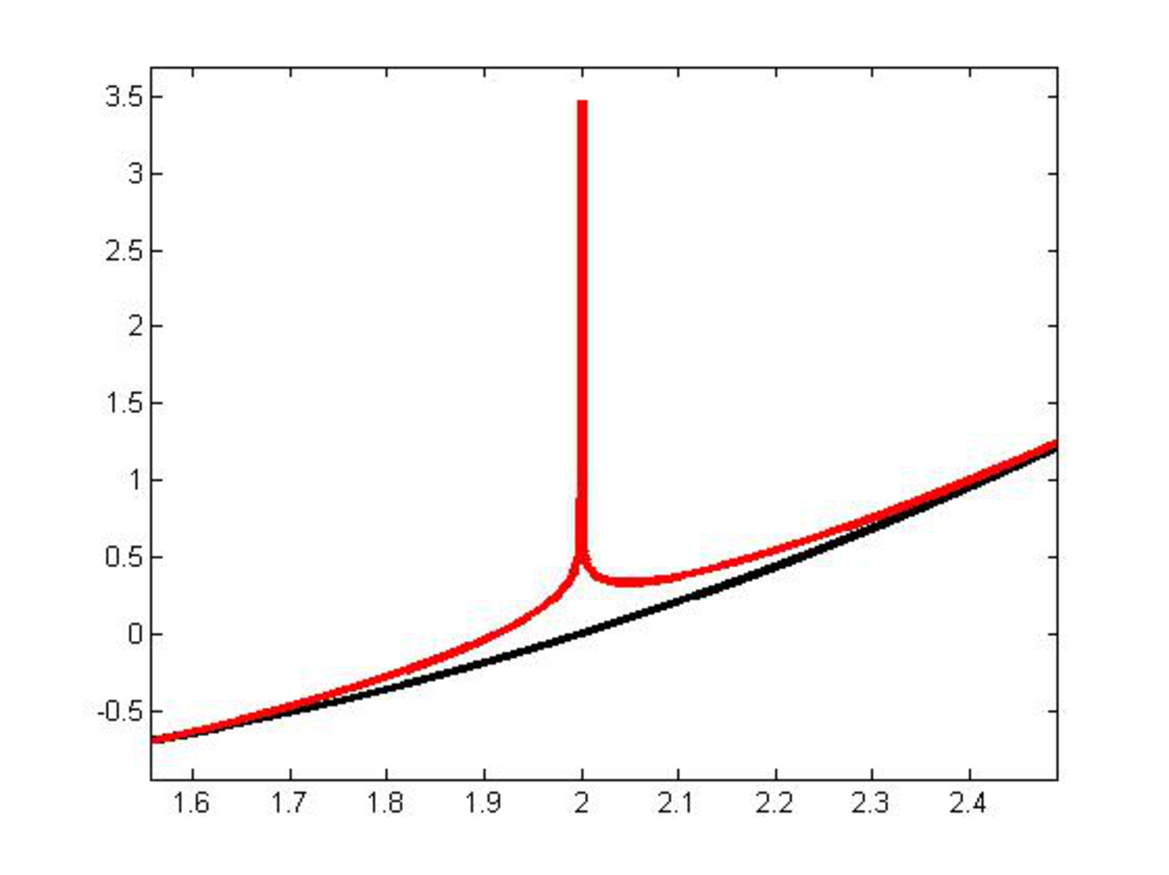
\includegraphics[width=6.0cm]{./images/ln-barrieren-u=0_1-2.pdf}
\end{minipage}
\\
\begin{minipage}[t]{1cm}
.
	\end{minipage}
\begin{minipage}[t]{6.0cm}
       $\mu = 1$
	\end{minipage}
	\hspace{0.1cm}
	\begin{minipage}[t]{6.0cm}	
			$\mu = 0.1$
	\end{minipage}
	\hspace{0.1cm}
	\begin{minipage}[t]{4.0cm}	
			$\mu = 0.1$ (Ausschnitt)
\end{minipage}


\newpage
\subsection{Der Algorithmus}

Für das Innere-Punkte-Verfahren gilt folgender, vereinfachter Algorithmus:
\\	
\begin{enumerate}
\item Wähle primale und duale Startvektoren $\vec{x},\vec{y},\vec{s} > 0$\\
\textit{ $\vec{x} =$ Startvektor primales Problem\\$\vec{y} = $ Startvektor duales Problem\\$\vec{s} =$ Startvektor Schlupfvariablen}\\
\item Setze $\mu = \vec{x^t} \cdot \vec{s}/n$\\
\textit{$\mu =$ Straftermparameter}\\
\item Reduziere $\mu_{neu}=\mu_{alt} \cdot (1-\frac{\beta}{\sqrt{n}})$ mit $\beta \in ]0;0.5[$\\
\textit{man kann beweisen, dass das Problem mit $\beta$ im Intervall (oben) immer konvergiert.}\\

\item Berechne die Newton-Richtung durch Lösen des linearen Gleichungssystem\\
$\begin{bmatrix}
0 & A^t & I \\ A & 0 & 0 \\ S & 0 & X \end{bmatrix}$ 
$\cdot$ 
$\begin{bmatrix} \Delta\vec{x}\\\Delta \vec{y}\\\Delta \vec{s} \end{bmatrix}$
 $=$                                                     
$\begin{bmatrix} \vec{c} - A^t \vec{y} - \vec{s} \\ \vec{b}-A\vec{x} \\ \mu_{neu}\vec{e}-XS\vec{e}
\end{bmatrix}$\\
\newline
\textit{$X,S$ ensprechen Diagonalmatrizen mit den Elementen der Vektoren $\vec{x}$, $\vec{s}$}\\
\textit{$\vec{c}$ = Zielvektor}\\
\textit{$\vec{b}$ = Vektor der Nebenbedingung}\\
\item Wähle eine Schrittweite $\alpha > 0$, so dass $\vec{x}+\alpha \cdot \vec{\Delta x} > 0$; $\vec{s}+\alpha \cdot \vec{ds} > 0$ komponentenweise gilt.\\
\textit{$\alpha = 1$ entspricht dem Kurzschrittverfahren}\\
\item Setze $\vec{x}_{neu} = \vec{x}_{alt}+\alpha \cdot \Delta \vec{x}, \vec{y}_{neu} = \vec{y}_{alt}+\alpha \cdot \Delta \vec{y}, \vec{s}_{neu} = \vec{s}_{alt}+\alpha \cdot \Delta \vec{s}$\\
\textit{der vorherige Punkt $X$ wird um $\Delta \vec{x}$ korrigiert, er wandert weiter Richtung Optimum}\\
\item Überprüfe die Genauigkeitsbedingung, wenn nicht erfüllt: zurück zu Punkt 3.\\
\textit{Bsp: $\mu$ kleiner als ein Grenzwert $\epsilon$}
\end{enumerate}



\subsection{Die Eigenschaften}
\subsubsection{Allgemein}
\begin{itemize}
	\item Das Innere-Punkte Verfahren ist global konvergent
	\item {Kurzschrittvariante ($\alpha = 1$) braucht am meisten Iterationen, im schlechtesten Fall rund $k=\sqrt{n} \cdot \frac{1}{\epsilon}$ Iterationen (n=Anzahl Schranken)}
	\item In Praxis werden rund log(n) Iterationen benötigt
\end{itemize}

\subsubsection{Vorteile}
\begin{itemize}
	\item weniger Iterationen bei grossen, dünn besetzten Problemen
	\item weniger Rechenaufwand und darum schneller
\end{itemize}

\subsubsection{Nachteile}
\begin{itemize}
	\item nicht so einfach zu verstehen wie Simplex-Algorithmus
	\item bei dick besetzten Problemen keine Vorteile zum Simplex-Algorithmus
	\item funktioniert nur bei regulären Matrizen
	\item Näherung der Lösung, Optimum der Berechnung für $n\mapsto \infty$ erhält man das exakte Optimum
\end{itemize}

\newpage
\subsection{Dimension des Problems vs. Zeit}
Ein Vergleich zur Effizienz der Algorithmen. Die dick besetzte Matrix ist vollständig mit Werten ungleich 0 besetzt, die dünn besetzte Matrix besteht zu 90 Prozent aus Nullen. rot = Inneres-Punkte-Verfahren; blau = Simplex-Algorithmus
\begin{minipage}[t]{9.0cm}
  \subsubsection{Zeit mit voll besetzter Matrix A}
  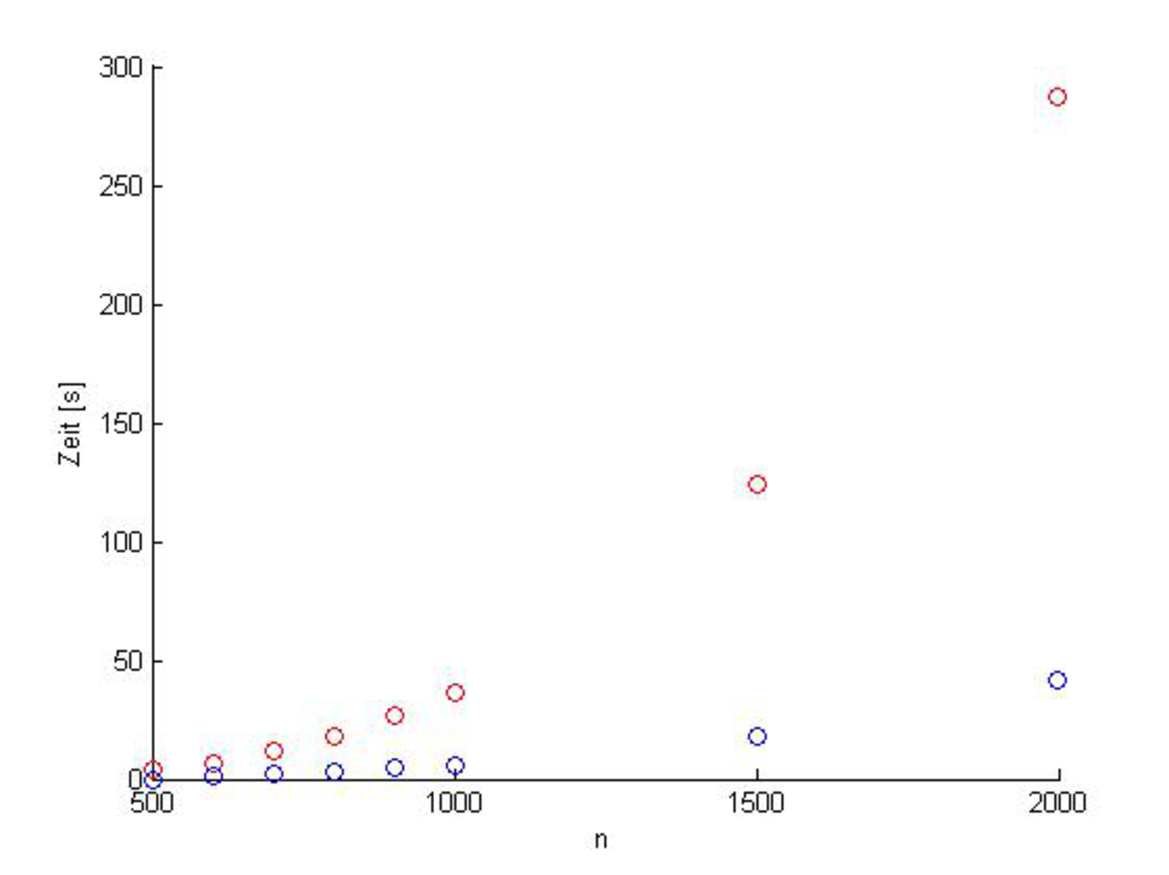
\includegraphics[width=8.5cm]{./images/dickbesetztematrix.pdf}
\end{minipage}
\hspace{0.1cm}
\begin{minipage}[t]{9.0cm}	
	\subsubsection{Zeit mit dünn besetzter Matrix A}
	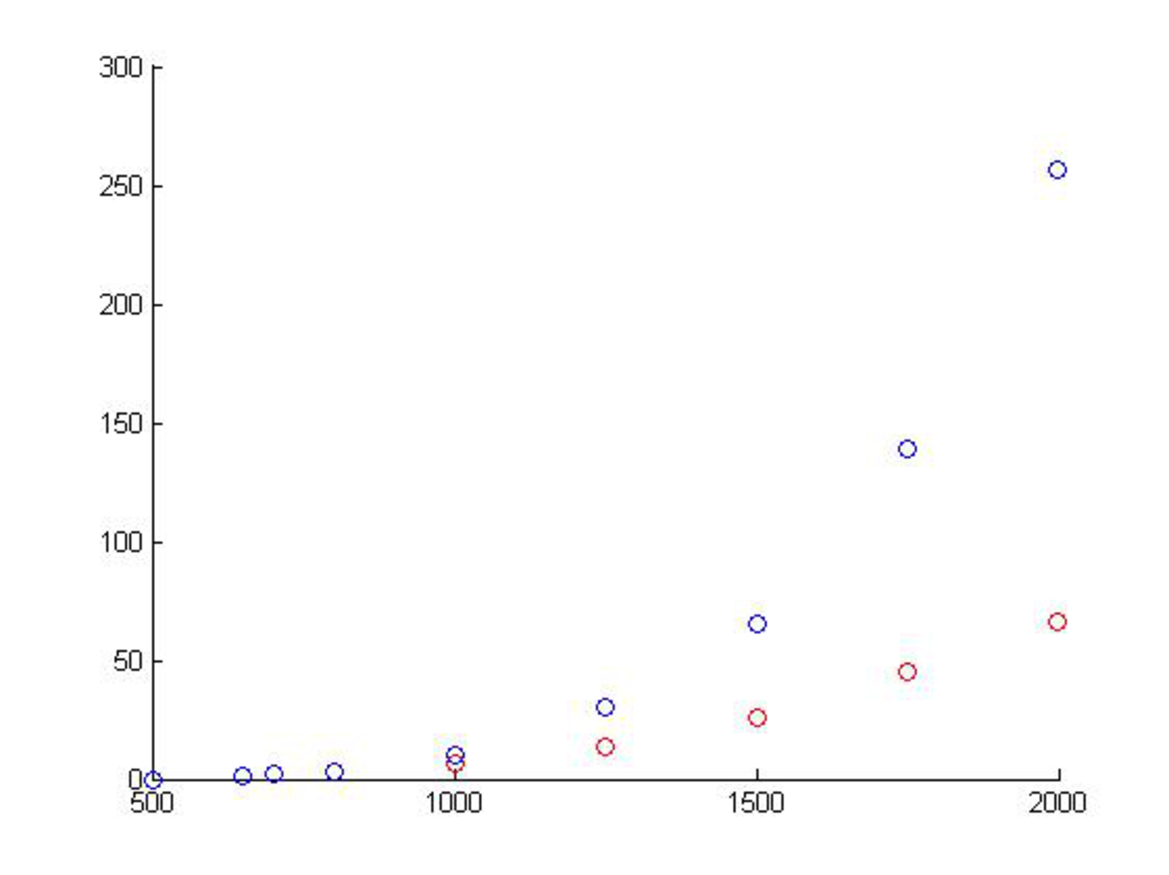
\includegraphics[width=8.5cm]{./images/duennbesetztematrix.pdf}
\end{minipage}



\subsection{Beispiel: Rosenbrock-Funktion}
An diesem Beispiel sieht man den verfolgten Pfad einer zweidimensionalen Funktion. Es wurde nicht der Kurzschrittalgorithmus verwendet, da von Punkt zu Punkt verschiedene Distanzen benützt wurden. Man kann sich das Prinzip für andere Probleme auch in 3 respektive n Dimensionen vorstellen.\\
 \\
$f(x_1, x_2) = 100 \cdot ((x_2+x_1^2)^2 + (1-x_1)^2)$\\
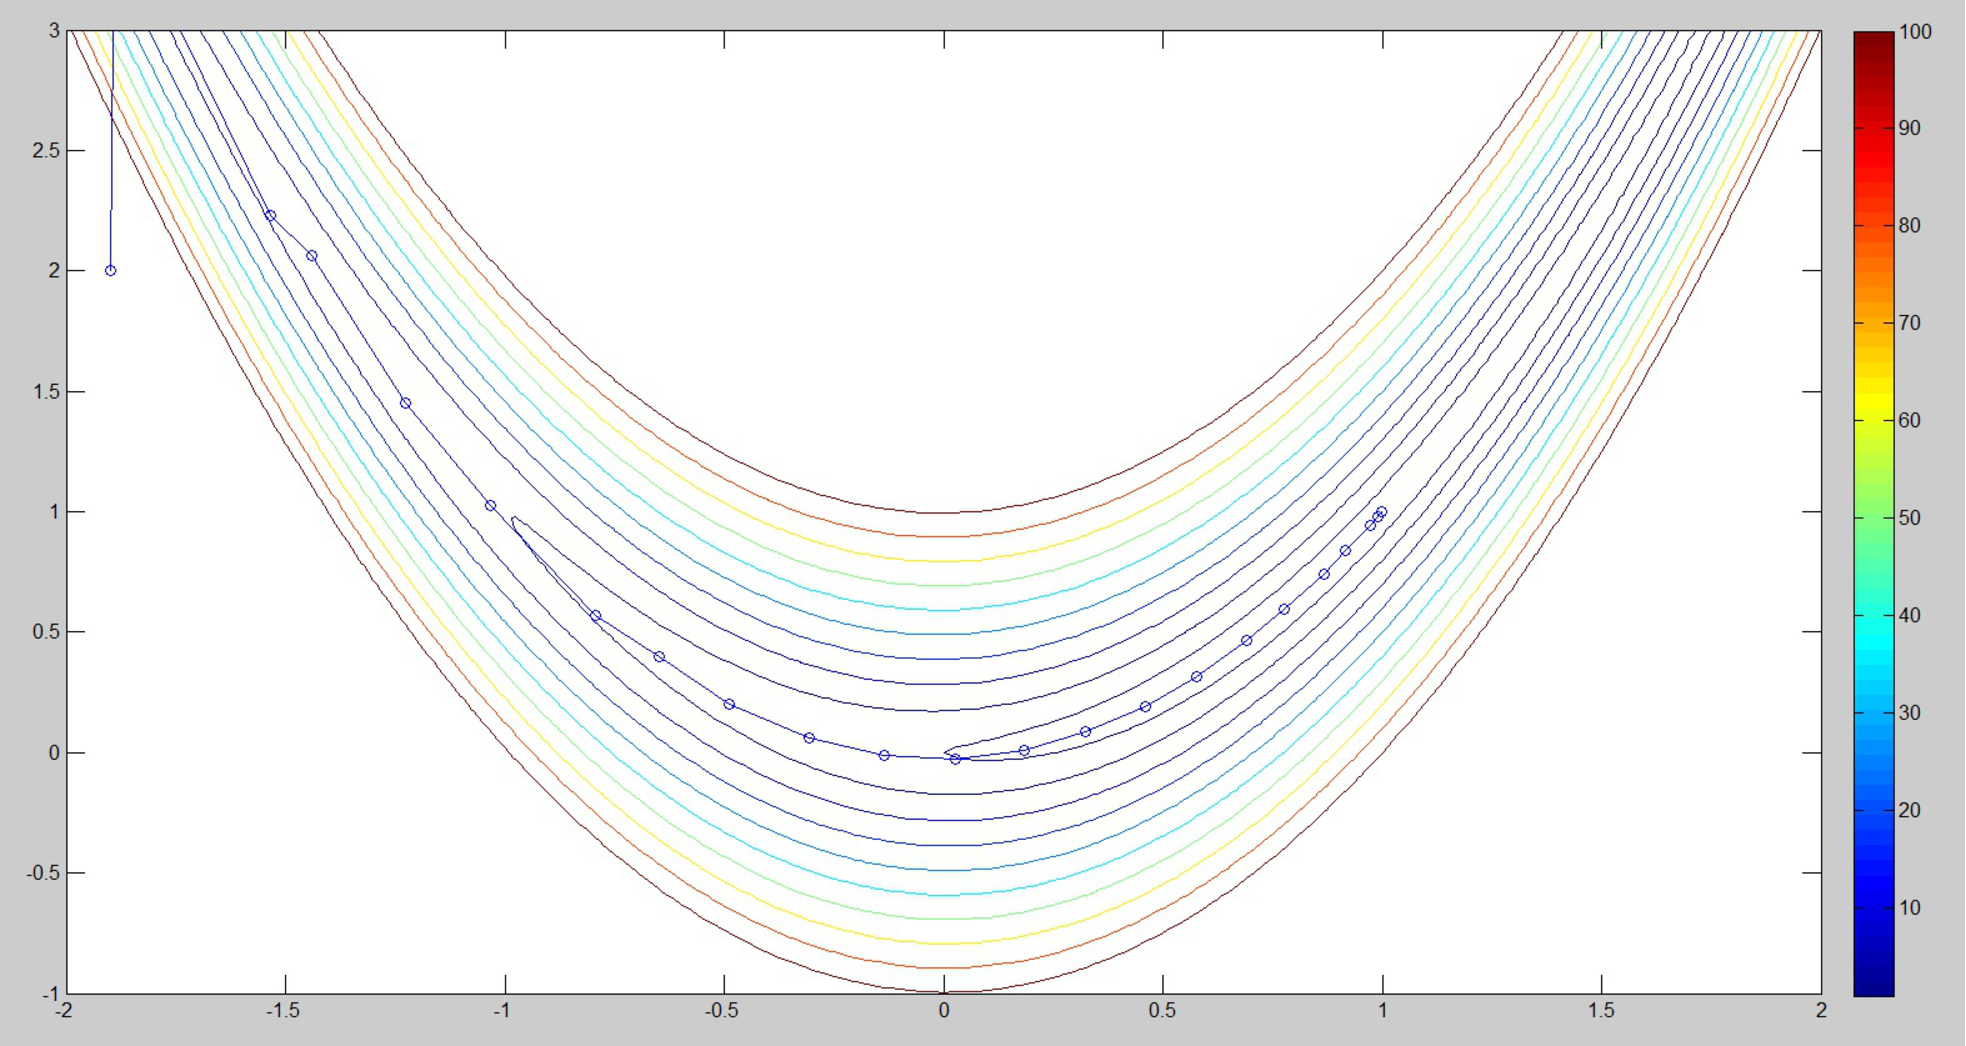
\includegraphics[width=18.0cm]{./images/Rosen.pdf}




\newpage

\subsection{Beispielcode}
\subsubsection{Code von Hand implementiert}
\begin{verbatim}
% bsp2.txt
% mathematisches Seminar FS 2013
% Optimierung: Innere-Punkte-Verfahren
% 20.04.2013

c =     [ 1,  6,  0,  3,  2]'             % Zielfunktion, zu minimieren

A =     [ 2,  2,  0,  0,  0;              % Matrix mit Nebenbedingungen
         -1,  0,  2,  2,  0;
          0, -1, -1,  0,  2;
          0,  0,  0, -1, -1]

b =     [5, 0, 0, -5]'                    % Vektor für Nebenbedingungen

e =     0.1*ones(5,1)                     % Genauigkeitsgrenze (Toleranz)																											
I =     eye(5)	

n =     4														
k =     1                                 % Iterationsvariable (Zähler)
a =     1                                 % Kurzschrittalgorithmus: Schrittweite = 1

%------------------------------------------ Schritt 1.)
x = 0.1*ones(5,1)                         % Startvektor für primales Problem
y = 0.1*ones(4,1)                         % Startvektor für duales Problem
s = 0.1*ones(5,1)                         % Startvektor für Schlupfvariablen

%------------------------------------------ Schritt 2.)
u = x'*s/n;

while u>0.001                             % Abbruchbedingung	

S = diag(s);                              % Diagonalmatrix mit Diagonalwerte von Vektoren x,s
X = diag(x);

% ------------------------------------------ Schritt 3.)
u=u*(1-(1/6)/sqrt(n));                    % neuer Straftermfaktor


% ------------------------------------------ Schritt 4.)
dxdyds = [zeros(5), A', I; A, zeros(4), zeros(4,5); S, zeros(5,4), X ]  \  [c-A'*y-s; b-A*x; u*e-S*X*e];


% ------------------------------------------ Schritt 5/6.)
x= x+a*[dxdyds(1), dxdyds(2), dxdyds(3), dxdyds(4), dxdyds(5)]';      % xneu = xalt + dx 
y= y+a*[dxdyds(6), dxdyds(7), dxdyds(8), dxdyds(9)]';                 % yneu = yalt + dy 
s= s+a*[dxdyds(10), dxdyds(11), dxdyds(12), dxdyds(13), dxdyds(14)]'; % sneu = salt + ds 

dx=[dxdyds(1), dxdyds(2), dxdyds(3), dxdyds(4), dxdyds(5)]';

k=k+1;                                    % Inkrementiere Variable k (Anzahl Durchläufe)

endwhile

k                                         % Ausgabe des k-ten Schritts
x                                         % Optimaler Punkt
\end{verbatim}


\vspace{0.1cm}

\newpage
\subsubsection{Code mit Hilfe von Octave-Funktion \textit{GLPK}}

\begin{verbatim}
% bsp2octave.txt
% mathematisches Seminar FS 2013
% Optimierung: Innere-Punkte-Verfahren
% 20.04.2013



c =     [ 1,  6,  0,  3,  2]'   % Zielfunktion, interpretieren als... (siehe Wert der Variable s)

A =     [ 2,  2,  0,  0,  0;
         -1,  0,  2,  2,  0;
          0, -1, -1,  0,  2;
          0,  0,  0, -1, -1]

b =     [5, 0, 0, -5]'
lb=     zeros(5,1)              % lower bound (=0, falls keine Untergrenze angegeben)
ub=     []                      % upper bound (=unendlich, falls keine Obergrenze angegeben)
ctype = "UUUU"                  % U = Ungleichung mit Obergrenze (b enthält grösstmögliche Werte)
vartype="CCCCC"                 % C = Continuous Variable; I = Integer Variable;
s =     1                       % -1 = Maximierungsproblem; 1 = Minimierungsproblem;

        
param.msglev =    3             % Parameter: Level of messages output by solver routines (1=no - 4=full)
param.itlim =     1000          % Parameter: Simplex max. Anzahl Iterationen
param.lpsolver = 	2             % Parameter: 1=Simplex / 2=innerePunkte

          
[xopt, fopt, status, extra] = glpk (c, A, b, lb, ub, ctype, vartype, s, param);


status                          % 150=innerPointMethod is undefined oder 151=innerPointMethod is optimal
extra                           % lambda=dual variables; redcosts = reduced costs; 
                                % time = time in seconds for LP/MIP problem; 
                                % mem = memory used for LP/MIP in bytes

		
xopt                            % Optimum, bester Punkt	
fopt                            % Wert des Optimums / des besten Punktes
\end{verbatim}

\subsection{Quellen}

\url{de.wikipedia.org/wiki/Innere-Punkte-Verfahren}\\
\url{www.gnu.org/software/octave/doc/interpreter/Linear-Programming.html}\\
\url{www.ruhr-uni-bochum.de/num1/files/theses/da_tunc.pdf}\\
\url{www.math.uni-hamburg.de/home/j.werner/kap4.pdf}\\
\url{www-m1.ma.tum.de/m1old/personen/sulbrich/opt3}
